\subsection{Thin-disk approximation}\label{analytic_relax}
Our final approximation apply to thin disks for 
which $\epsilon\ll 1$. Then we may write $\rho/\rho_0\simeq
\exp{(-\zhat^2/2)}$. The governing equation,
Eq. \ref{vertiso_gov_nondim}, is then   
\begin{align}
  \delta v_z^{\prime\prime} - z A\delta v_z^\prime +
  (B - C\zhat^2)\delta v_z = 0,\label{nearly_iso_explicit}
\end{align}
with
\begin{align}
  &A \equiv 1 + \ii \epsilon q \hat{k},\\
  &B \equiv \hat{\sigma}^2\left(\chi + \hat{k}^2\right) -
  \left(\chi + \ii \epsilon q \hat{k}\right),\\
  &C \equiv \left(1-\chi\right)\left(\hat{k}^2 - \ii
    \epsilon q\hat{k}\right), 
\end{align}
and $\chi =
\left(1-\ii\hat{\sigma}\beta\right)/\left(1-\ii\hat{\sigma}\beta\gamma\right)
$ in terms of dimensionless variables. 

We remark that Eq. \ref{nearly_iso_explicit} is in the same 
form as Eq. 41 in \cite{lubow93}, which describe adiabatic axisymmetric waves in
a vertically isothermal disk without vertical shear. The two equations
become identical after  setting $q=0$ (no vertical shear) and
$\chi=1/\gamma$ (adiabatic flow) in our Eq. \ref{nearly_iso_explicit},
and making the low-frequency, nearly-Keplerian approximation in
\citeauthor{lubow93} after a change of variables.    

% The thin disk approximation allows us to develop explicit solutions,
% but some general results may be established without it (see,
% e.g. Appendix \ref{global_corr} and \S\ref{iso_pert}).     

\subsection{Isothermal perturbations}\label{iso_pert}
Isothermal perturbations correspond to $\beta = 0$ or $\chi = 1$. This
case has been investigated numerically by \cite{nelson13} and 
\cite{mcnally14}, the latter of which employed the VGSB framework.  

In Appendix \ref{iso_discuss}, we give an analytical discussion of the
linear problem with $\beta=0$. There, we establish more general
results that do not require the thin disk approximation, namely 
a necessary condition for instability (there must be vertical shear)
and an upper bound to the instability growth rate (it is limited by
the maximum vertical shear rate in the disk). We also develop analytic
solutions in the thin disk limit. The methods used in Appendix
\ref{iso_discuss} and results obtained therein motivates the solution
procedure employed in the following sections.      

\subsection{The effect of introducing a small but finite
  thermal relaxation time}\label{relax_pert}
We are interested in the case $\beta\neq 0$, but it is instructive to
first ask  the more analytically tractable question: how 
do the eigenfrequencies and eigenfunctions change when we change
$t_c=\beta\Omega_k^{-1}$ from zero to a small but finite value? For 
sufficiently small $\beta$ % , for which the perturbations may be 
% considered nearly-isothermal,
we expect the solution to only differ slightly from a case with
$\beta\equiv 0$. We thus perturb a solution for $\beta=0$ to see the
effect of thermal relaxation.  

For definiteness, let us consider the simple solution 
\begin{align}
  \beta\equiv 0, \quad \delta v_z = 1,\quad \hat{\sigma}^2 = \frac{1 +
  \ii\epsilon q \hat{k}}{1+\hat{k}^2}, \label{pert_basic} 
\end{align}
which solves Eq. \ref{nearly_iso_explicit} since $\delta
v_z=$constant and $\chi=1$ so that $B=C=0$. 
This is the fundamental or `corrugation' mode and represents
the entire disk column moving vertically. These modes have been
observed to dominate numerical simulations \citep{nelson13,stoll14},
and are the ones we find to develop in protoplanetary disks
with a realistic estimate for thermal timescales
(\S\ref{application}). 

%To determine the (assumed) small effect of introducing a short thermal
%relaxation, 
We linearize Eq. \ref{nearly_iso_explicit} about the above
solution for $\beta\equiv0$ and write 
\begin{align}\label{nearly_iso_pert}
  \beta \to 0 + \delta\beta,\, \delta v_z\to \delta v_z+\delta
  v_{z1},\,\hat{\sigma} \to \hat{\sigma} + \delta\hat{\sigma}, 
\end{align}
which implies 
\begin{align}
  \chi \to 1 + \delta\chi = 1 + \ii \hat{\sigma}\left(\gamma-1\right)\delta\beta,
\end{align}
with $\delta v_z$ and $\hat{\sigma}$ given by Eq. \ref{pert_basic}. We
may then seek  
\begin{align}
  \delta v_{z1} = a \zhat^2 + b,
\end{align}
where $a$, $b$ are constants. 

Inserting Eq. \ref{nearly_iso_pert} into Eq. \ref{nearly_iso_explicit}
and keeping only first order terms yield the requirements, after
balancing constants and coefficients of $\zhat^2$, 
% we obtain  
% \begin{align}
%  0 =& \delta v_{z1}^{\prime\prime} - z\left(1 + \ii\epsilon q
%    k\right)\delta v_{z1}^\prime\notag\\
%  &+ \left[2\hat{\sigma}\delta\hat{\sigma}\left(1 + \khat^2\right) +
%    \left(\hat{\sigma}^2 - 1\right)\delta\chi \right.\notag\\
% &\phantom{++} \left. + \zhat^2\left(\khat^2 -
%      \ii\epsilon q \khat\right)\delta\chi\right]\delta v_z\notag\\
%  &+\left[\hat{\sigma}^2\left(1 + \khat^2\right) - \left(1+\ii\epsilon
%      q \khat\right)\right]\delta v_{z1}.\label{nearly_iso4}
% \end{align}
% In Eq. \ref{nearly_iso_pert} and \ref{nearly_iso4}, $\delta v_z$ is to
% a solution to Eq. \ref{nearly_iso_explicit} with 
% $\beta=0$. 
% We could proceed by considering the entire set of polynomial solutions
% for $W$, and hence for $\delta v_z$, as derived in \S\ref{iso_poly}, but it
% is simplest to look at the fundamental mode. 
%Inserting the above expressions for $\delta v_z$, $\delta v_{z1}$ and
%$\hat{\sigma}^2$ into Eq. \ref{nearly_iso4}, then balancing
%coefficients of $\zhat^2$ and constants, we require
\begin{align}
  0 &= 2a + 2\hat{\sigma}\left(1+\khat^2\right)\delta\hat{\sigma} +
  \left(\hat{\sigma}^2 -1\right)\delta\chi,\notag\\
  0&= 2a\left(1+\ii\epsilon q \khat\right) - \left(\khat^2 - \ii\epsilon
    q \khat\right)\delta\chi.
\end{align} 

Using the expressions for $\delta\chi$ and $\hat{\sigma}$ we can solve
for $\delta\hat{\sigma}$. This gives 
\begin{align}\label{nearly_iso_dsig}
  \delta \hat{\sigma} =
  -\frac{\ii\left(\gamma-1\right)\hat{k}^2\left(\ii\epsilon
      q - \hat{k}\right)^2}{2\left(1+\ii\epsilon q \hat{k}\right)\left(1+\hat{k}^2\right)^2}\delta\beta.
\end{align}
The imaginary part of Eq. \ref{nearly_iso_dsig} is
\begin{align}
  \delta\hat{\nu} =
  -\frac{\left(\gamma-1\right)\hat{k}^2 \left(\hat{k}^2 -
      2\epsilon^2q^2\hat{k}^2 - \epsilon^2q^2\right)}{2\left(1+\epsilon^2 q^2
      \hat{k}^2\right)\left(1+\hat{k}^2\right)^2}\delta\beta.  
\end{align}
Since $\epsilon \ll 1$, introducing finite cooling $\delta\beta>0$
implies $\delta\hat{\nu} < 0$, i.e. stabilization. Interestingly, for both
$\hat{k}\to0$ and $\hat{k}\to\infty$ we find $\delta\hat{\nu}\to0$, so
stabilization by small finite cooling is ineffective at very large or
very small scales. 
% We plot Eq. \ref{nearly_iso_dsig} in
% Fig. \ref{domegadbeta} with 
% $\epsilon=0.05$, $q=-1.0$ and $\gamma=1.4$. For this disk model the
% optimum wavenumber for stabilization is $\hat{k}\sim 5$---$6$.  

% This contrasts to the case without vertical shear
% ($q=0$), in which $\p\hat{\sigma}/\p\beta\to\mathrm{constant}$ as 
% $\hat{k}\to\infty$.  

% \begin{figure}
%   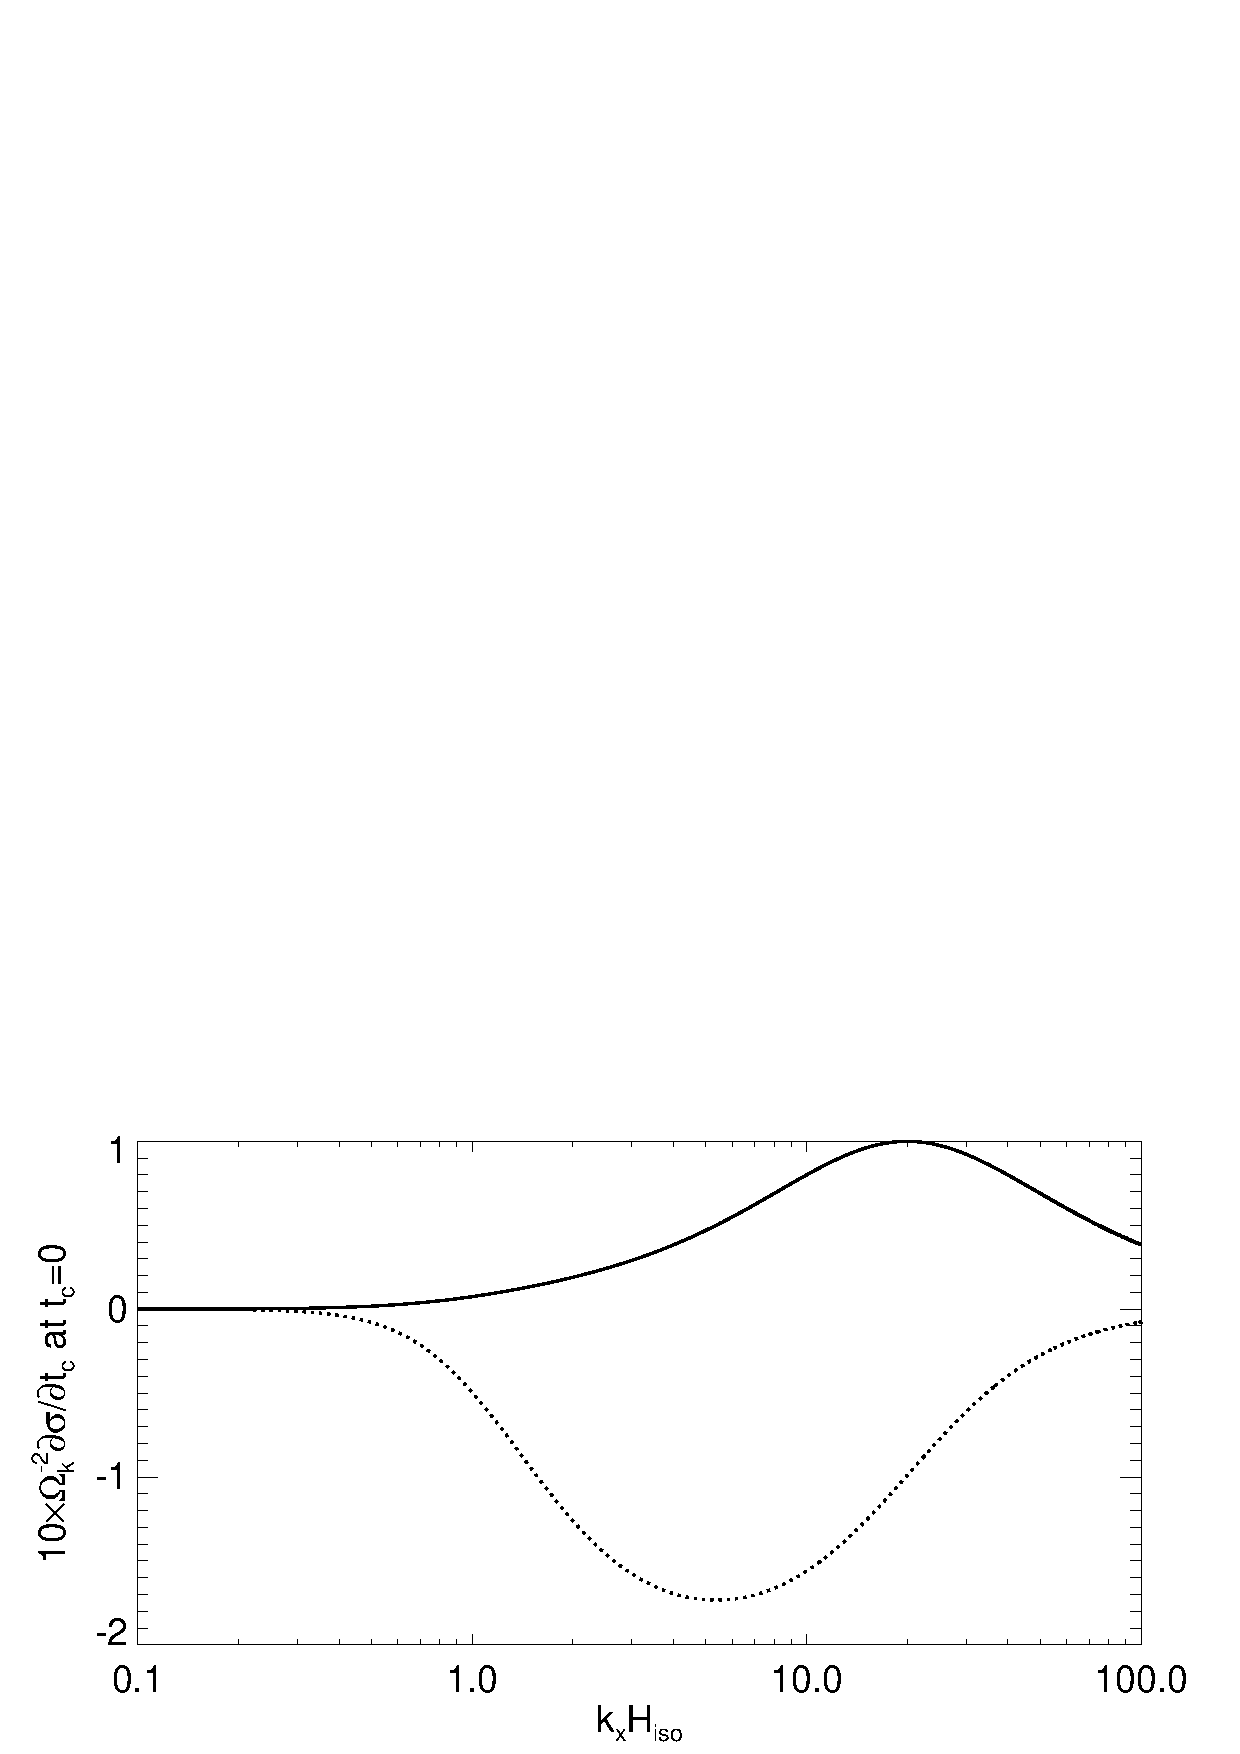
\includegraphics[width=\linewidth]{figures/domegadbeta}
%   \caption{Rate of change of the fundamental VSI eigenfrequency
%   $\sigma$ with respect to the introduction of a small but finite
%   cooling time. The plotted quantity is $\p\hat{\sigma}/\p\beta$ at $\beta=0$, evaluated using
%   Eq. \ref{nearly_iso_dsig} with 
%   disk parameters $\epsilon=0.05$, $q=-1$ and $\gamma=1.4$. The real
%   (imaginary) part of $\p\hat{\sigma}/\p\beta$ is shown as the solid
%   (dotted) lines. 
%   \label{domegadbeta}}  
% \end{figure}   

A finite thermal relaxation time introduces buoyancy
forces, which is stabilizing for sub-adiabatically stratified disks
($\gamma > 1$). The $\zhat^2$ dependence in $\delta v_{z1}$ then makes
sense because it becomes significant for large $|\zhat|$, i.e. away from
the midplane where the effect of buoyancy first appears as $\beta$ is
increased from zero. 

\subsection{Explicit solutions and dispersion relation}\label{disp_relax}
%To obtain a dispersion relation similar to that for 
%isothermal perturbations (Eq. \ref{sig2_iso}), 
We now solve Eq. \ref{nearly_iso_explicit} explicitly. We first write  
\begin{align}
  \delta v_z(\zhat) =
  g(\zhat)\exp\left(\frac{\alpha\zhat^2}{2}\right), \label{adia_ansatz}
\end{align}
where $\alpha$ is a constant to be chosen for convenience. Inserting
Eq. \ref{adia_ansatz} into Eq. \ref{nearly_iso_explicit} gives
\begin{align}
  0 = g^{\prime\prime} - \hat{z}\left(A - 2\alpha\right)g^\prime + \left(B +
    \alpha\right)g
  +\left(\alpha^2 - \alpha A - C\right)\zhat^2 g.
\end{align}
We choose $\alpha$ to make the coefficient of $\zhat^2g$
vanish, and impose the vertical kinetic energy density
$\rho|\delta v_z|^2\propto |g|^2 \exp{\left(\real\alpha -
    1/2\right)\zhat^2}$ to remain finite as $|\zhat|\to\infty$. 
Then assuming $g(\zhat)$ is a polynomial, we require  
\begin{align}
  \real\alpha < \frac{1}{2}, 
\end{align}
which amounts to choosing 
\begin{align}
  \alpha = \frac{1}{2}\left(A - \sqrt{A^2 + 4C}\right).  
\end{align} 
%by considering the case $q=0$ and $\beta\to\infty$ as examined in
%\cite{lubow93}.   

Eq. \ref{nearly_iso_explicit} becomes 
\begin{align}
  0 = g^{\prime\prime} - \hat{z}\left(A - 2\alpha\right)g^\prime +
  \left(B + \alpha\right)g.
\end{align}
We seek polynomial solutions 
\begin{align}
  g(\zhat) = \sum_{m=0}^M b_m \zhat^m,
\end{align}
which requires
\begin{align}
  B(\hat{\sigma}) + \alpha(\hat{\sigma}) =
  M\left[A-2\alpha(\hat{\sigma})\right].\label{adia_disp0} 
\end{align}
% We remark that for $q=0$ and $\beta\to\infty$, Eq. \ref{adia_disp0} is
% the same as Eq. 54 in \cite{lubow93} when the low-frequency, Keplerian
% approximation is made in the latter. 
% Eq. \ref{nearly_iso_explicit} is same form
% as the governing equation for the adiabatic case
% (Eq. \ref{adia_iso4}). However, the coefficients $\widetilde{B}$ and $\widetilde{C}$
% have a complicated dependence on $\hat{\sigma}$. 
% Applying the same solution method as in \S\ref{adia_explicit}, we 
% find the adiabatic dispersion relation, 
This is a $6^\mathrm{th}$ order 
polynomial in $\hat{\sigma}$:  
\begin{align}
  0 = \sum_{l=0}^{6}c_l\hat{\sigma}^l,\label{relax_disp}
\end{align}
where the coefficients $c_l$ are given in Appendix \ref{relax_coeff}.
The dispersion relation $\hat{\sigma}=\hat{\sigma}(\khat)$ generally
requires a numerical solution. However, for the fundamental mode
($M=0$) some analytic progress can be made, which we consider next.  

% It is simplest to solve Eq. \ref{relax_disp} numerically. In
% Fig. \ref{relax_disp_fig} we plot the growth rate of the fundamental
% ($M=0$) VSI mode as a function of $\khat$ for a range of
% dimensionless thermal relaxation timescales $\beta$, in a disk with
% $\epsilon=0.05$, $q=-1$ and $\gamma=1.4$. Increasing $\beta$ even
% slightly above zero significantly reduces the growth rates for
% $\khat\gg 1$. (There is little effect at small $\khat$ but this case is
% not of interest because the local model breaks down.) Thus, 
% a growing fundamental VSI mode exists only for nearly
% isothermal perturbations ($\beta\ll 1$).  The plot is also consistent with our previous
% discussion that there exists an intermediate wavenumber for which
% finite thermal relaxation has maximal effect (for small $\beta$). 

% \begin{figure}
%   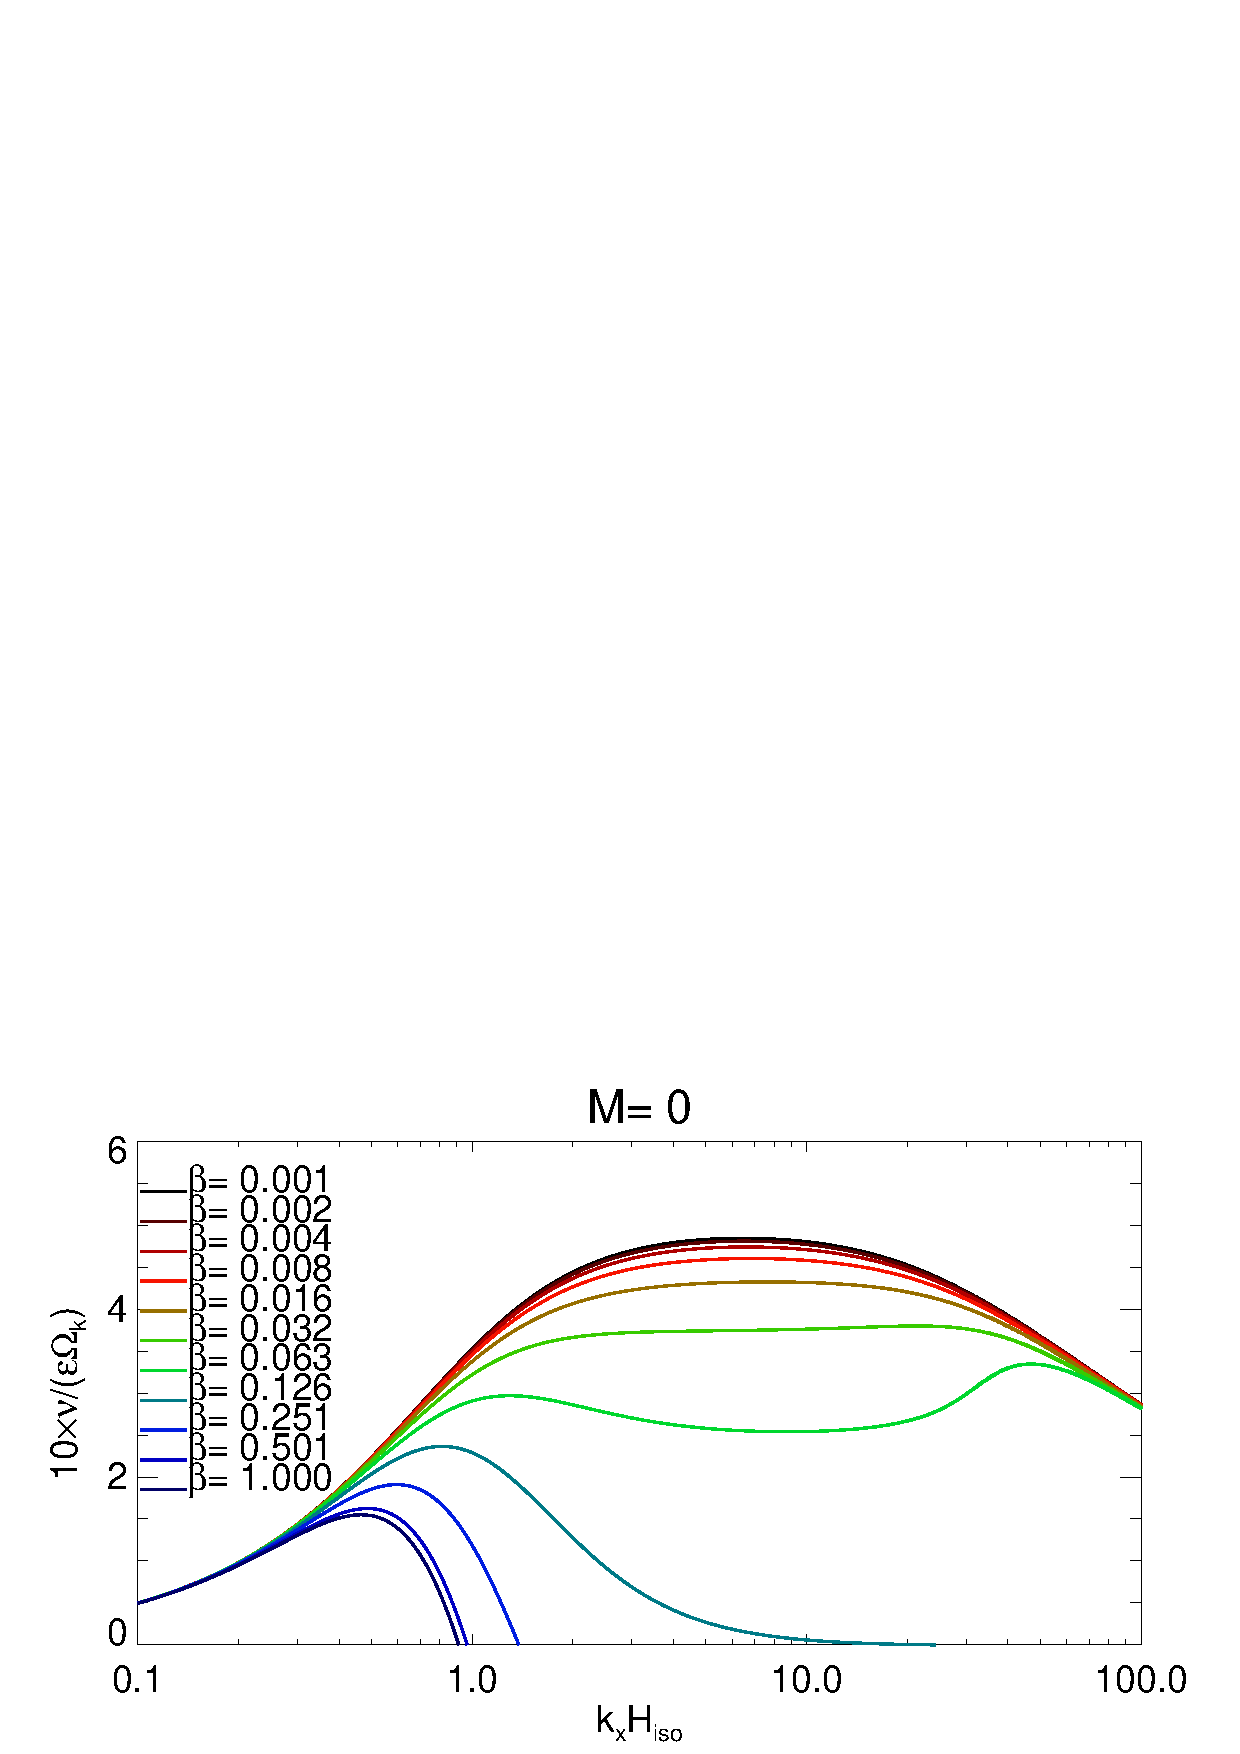
\includegraphics[width=\linewidth,clip=true,trim=0cm 0.0cm 0cm 0cm]{figures/rate_theory_grow_relax}
% %  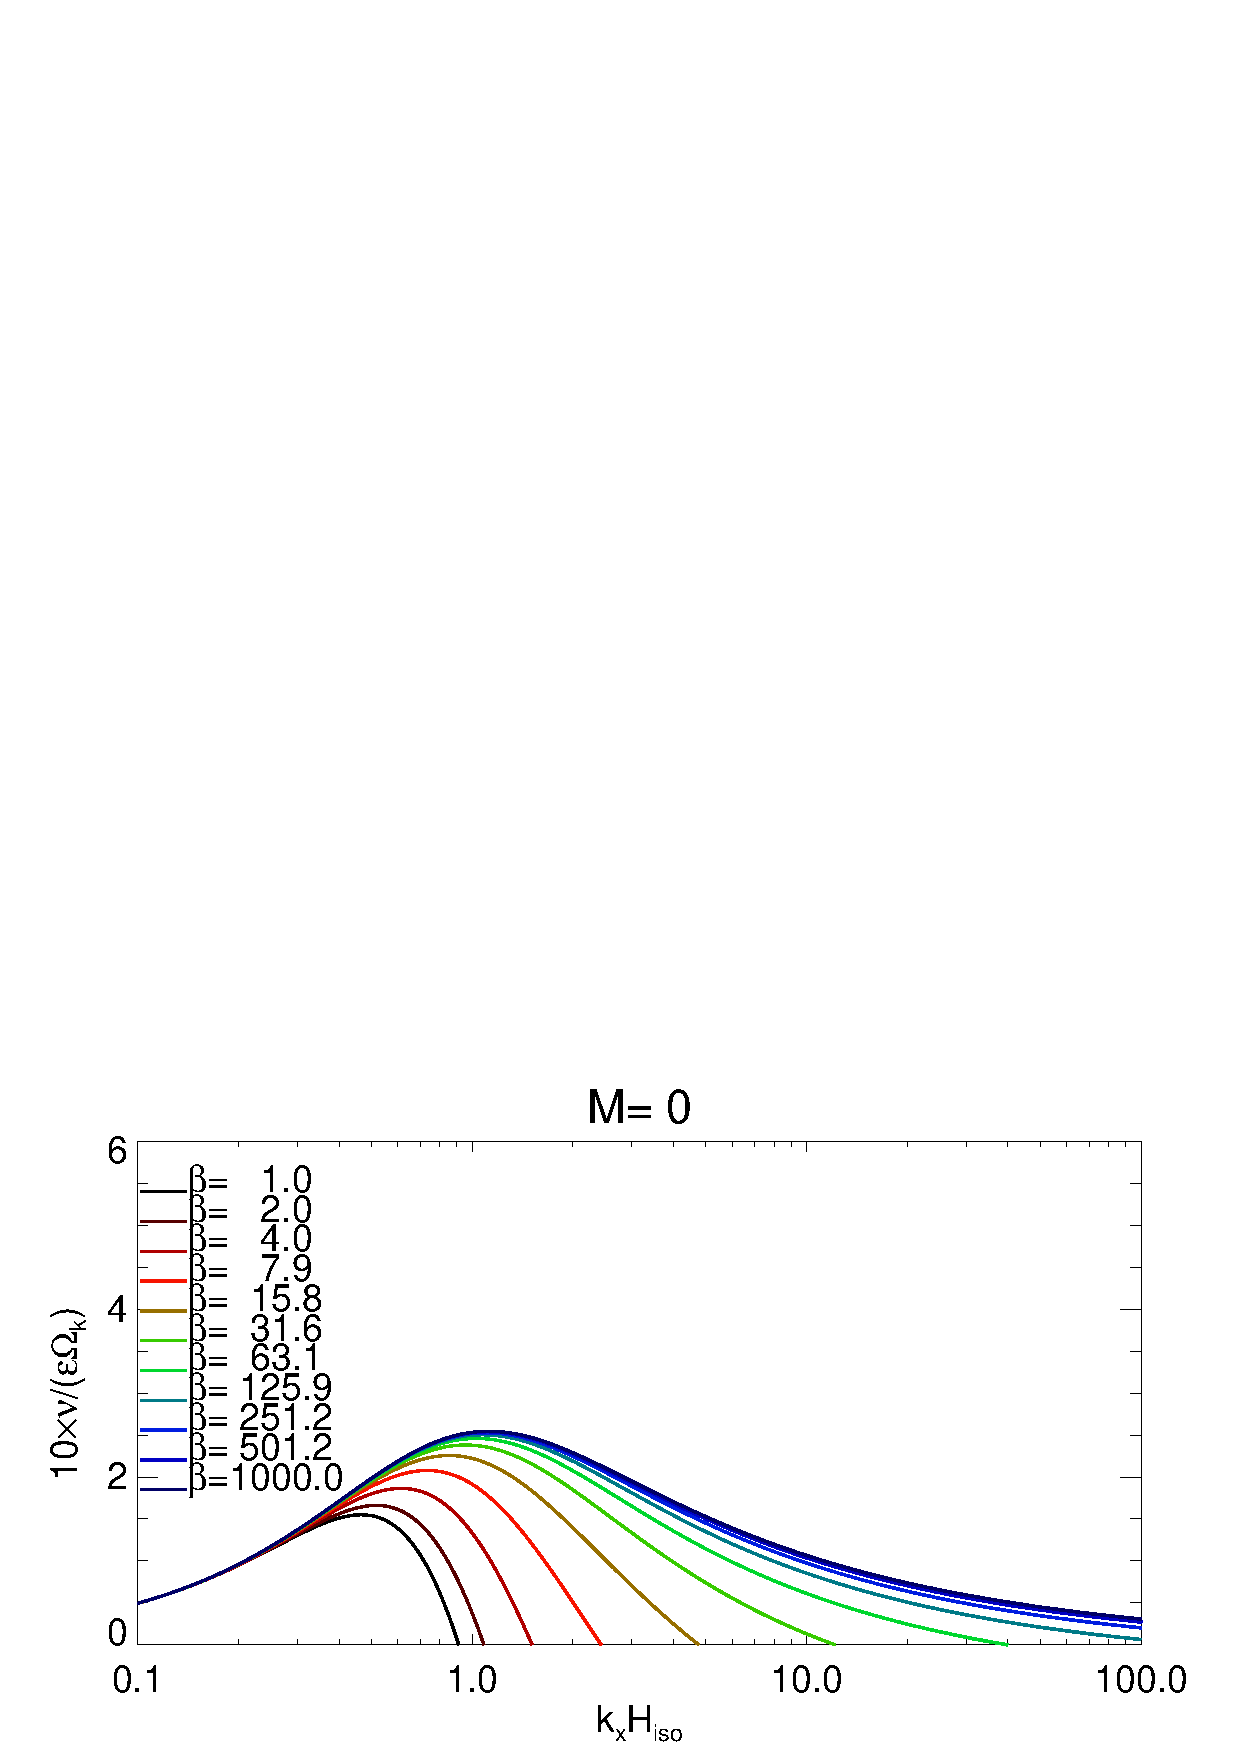
\includegraphics[width=\linewidth,clip=true,trim=0cm 0cm 0cm 1cm]{figures/rate_theory_grow_relax2}
%   \caption{Growth rate of the fundamental VSI mode in a disk with
%     dimensionless thermal relaxation timescales
%     $\beta\in[10^{-3},1]$.  Other disk parameters are
%     $\epsilon=0.05$, $q=-1$ and $\gamma=1.4$. The growth rates are
%     calculated from the dispersion relation Eq. \ref{relax_disp}. 
%     \label{relax_disp_fig}}  
% \end{figure}   

% ate_theory, eps=0.05, smallq=-1d0, gmma=1.4, bmax=1.0, ncases=11,
%mmode=0.0, root=1, legend=[0.102,0.14,5.4,0.355], yrange=[0,6]

\subsection{Upper limit on the thermal relaxation timescale for the
  fundamental VSI mode}\label{iso_vsi_beta_crit}

Here we estimate the maximum thermal relaxation timescale
$\beta$ that allows the fundamental VSI mode for $\khat\gg1$.   
% Notice in Fig. \ref{relax_bcrit} the upper limit on $\beta$ for the
% fundamental isothermal VSI tends to a constant for large
% $\khat$. Using this clue, we can calculate this critical $\beta$ by
% considering $\khat\to\infty$. We proceed as follows. 
At marginal stability, the eigenfrequency $\hat{\sigma}=\hat{\omega}$
is real. The dispersion relation for the fundamental mode is then
\begin{align}\label{relax_disp_fund}
  0 = \sum_{l=1}^{6}c_l\hat{\omega}^l \quad \text{for $M=\hat{\nu}=0$}.  
\end{align} 
Taking the real and imaginary parts of Eq. \ref{relax_disp_fund} and considering 
$\khat\gg1$, we find
\begin{align}
  0 =& \left[1 + \gamma\beta^2\left(1-\gamma\right)\right] + 2\epsilon q
  \gamma\beta (\hat{\omega}\khat) -  (\hat{\omega}\khat)^2 \notag\\
  &+ \beta^2\gamma^2\hat{\omega}^2 (\hat{\omega}\khat)^2,\label{relax_cond1}\\
  0=& \beta(1-\gamma)\khat^2 + \epsilon q \khat^2 (\hat{\omega}\khat)
  - 2\beta (\hat{\omega}\khat)^2 - \epsilon q \gamma^2\beta^2 (\hat{\omega}\khat)^3 \notag\\
    &+ 2\beta\gamma(\hat{\omega}\khat)^4.  
\label{relax_cond2}
\end{align}
This is a pair of simultaneous equations for
$\hat{\omega}$ and $\beta$. In Appendix \ref {iso_stable} we discuss
stable solutions without vertical shear which yield
$\hat{\omega}\propto \khat^{-1}$ for $\khat\gg 1$
(Eq. \ref{iso_stable_disp}).  We are thus motivated to seek solutions
to Eq. \ref{relax_cond1}---\ref{relax_cond2} with  
% we wish to seek a criterion independent of k 
% \begin{align}
%   \khat \to \infty, \quad \hat{\omega}\to 0 ,\quad \hat{\omega} \khat\text{ finite}.
%\end{align}
\begin{align}
  \khat \gg1, \quad |\hat{\omega}|\ll 1 ,\quad
  |\hat{\omega}\khat|=O(1). 
\end{align}
Then
\begin{align}
  \hat{\omega}\khat = \frac{(\gamma-1)\beta}{\epsilon q}
\end{align}
from Eq. \ref{relax_cond2}, which implies, from Eq. \ref{relax_cond1}
that
\begin{align}\label{beta_crit0}
  \beta = \frac{1}{(\gamma-1)}\left[\frac{1}{\left(\epsilon
        q\right)^2} - \frac{\gamma}{(\gamma-1)}\right]^{-1/2} 
\end{align}
at marginal stability for perturbations with large $\khat$. 

From our discussion in \S\ref{relax_pert}, which indicate introducing
a finite thermal relaxation is stabilizing, we expect
Eq. \ref{beta_crit0} is an upper limit. For a thin  
disk $\epsilon\ll 1$, we thus infer 
\begin{align}\label{iso_vsi_cond}
  \beta \lesssim \frac{|\epsilon q|}{\gamma-1} \equiv
  \beta_\mathrm{crit} 
\end{align}
is required for the fundamental VSI to operate. That is, when
$\beta<\beta_\mathrm{crit}$, perturbations are  effectively isothermal. 
We will confirm Eq. \ref{iso_vsi_cond} numerically in
\S\ref{bcrit_num_test}. 

Rapid thermal relaxation is required to overcome a stabilizing
vertical entropy gradient \citep{goldreich67,urpin98,urpin03}, but
this conclusion was reached in these studies by considering
vertically-localized disturbances. % , although a definitive timescale
                                % was not presented.  
By contrast, our Eq. \ref{iso_vsi_cond} quantifies this requirement
for vertically global disturbances (i.e. the fundamental mode). We see
that in a thin disk, a very short thermal timescale
 is required ($\beta_\mathrm{crit}\ll 1$) because
$\beta_\mathrm{crit}\propto \epsilon$. 
This suggests that
finite thermal relaxation rapidly stabilizes the VSI.  




% In Fig. \ref{relax_bcrit} we plot the critical thermal relaxation
% timescale obtained from solving Eq. \ref{relax_disp_fund} numerically 
% for a disk with $\epsilon = 0.05$, $q=-1$ and $\gamma=1.4$, for which
% we have $\beta_\mathrm{crit}=0.125$ from Eq. \ref{iso_vsi_cond}. Our
% upper estimate agrees well with the numerical solution for $\khat\gtrsim
% 10$. 

% \begin{figure}
%   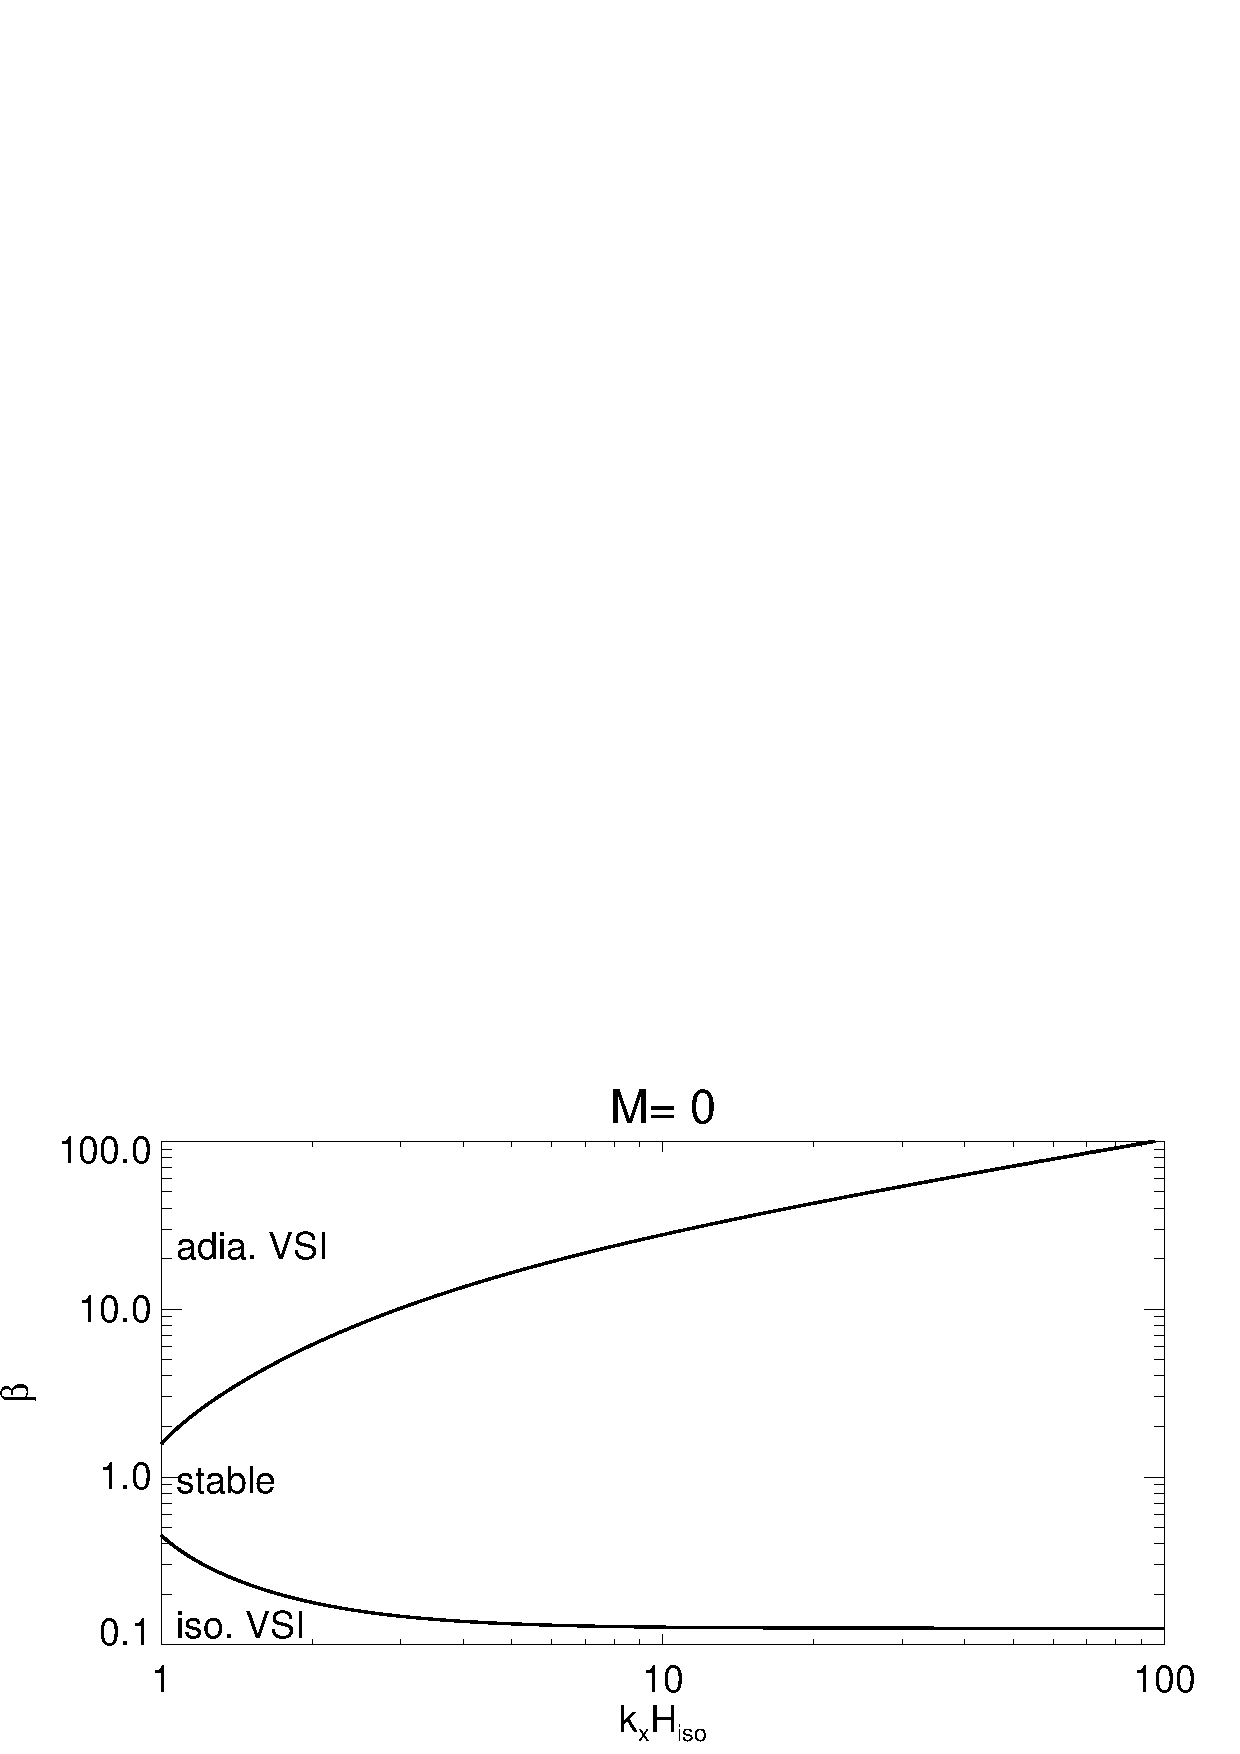
\includegraphics[width=\linewidth]{figures/bcrit_theory}
%   \caption{Condition on the thermal relaxation timescale $\beta$ for
%     the existence of unstable fundamental VSI mode in a vertically
%     isothermal disk with $\epsilon=0.05$, $q=-1$ and $\gamma=1.4$.  
%     The dotted line denotes the asymptotic value
%     $\beta_\mathrm{crit}=\epsilon|q|/(\gamma-1)$ for large $\khat$. 
%     \label{relax_bcrit}}  
% \end{figure}   



% \subsubsection{Lower limit on the thermal relaxation timescale for the
%   fundamental adiabatic VSI mode}
% {\bf Note: for reference only. Not to be included in paper.} 
% Fig. \ref{relax_bcrit} indicates there exists a lower limit on the
% thermal relaxation time for the system to behave adiabatically and
% support the fundamental adiabatic VSI. This critical
% timescale satisfies Eq. \ref{relax_cond1}---\ref{relax_cond2} with 
% \begin{align}
%   \beta \sim \beta_0\khat^{1/2},\quad \hat{\omega}  \sim
%   \hat{\omega}_0\khat^{-1/2} \text{ as } \khat\to\infty.
% \end{align}
% The constants $\beta_0$ and $\hat{\omega}_0$ are determined by the
% simultaneous equations
% \begin{align}
%   & 0 = \gamma\beta_0^2(1-\gamma) + 2\epsilon q \gamma
%   \beta_0\hat{\omega}_0 - \hat{\omega}_0^2 +
%   \beta_0^2\gamma^2\hat{\omega}_0^4.\\
%   & 0= \beta_0(1-\gamma) + \epsilon q \hat{\omega}_0 - \epsilon q
%   \gamma^2 \beta_0^2\hat{\omega}_0^3. 
% \end{align}
% For $\epsilon = 0.05$, $q=-1$ and $\gamma=1.4$, the appropriate
% solution is $\beta_0 = 10.33$ and $\hat{\omega}_0 = 0.74$.  





% If we follow through the solution method as before, we obtain a
% dispersion relation 
% \begin{align}
%   &\hat{\sigma}^2\left(\frac{1}{\gamma}+\hat{k}^2\right) \notag\\ &=
%   \left(\frac{1}{\gamma}-\frac{1}{2}\right) +\frac{\ii}{2}\epsilon q
%   \hat{k} + \frac{1}{2}\left(2M+1\right)\left(A^2 + 4C\right)^{1/2}\label{adia_disp}.
% \end{align}
% This equation is the same as Eq. 54 in \cite{lubow93} when $q=0$ and
% the low-frequency, Keplerian approximation is made for the latter.  



% Note that when $\gamma>1$ and $q=0$, the term with $\ln\rho^{\prime
%   2}$ in the integrand (third term on the RHS) represents
% stabilization by the vertical entropy gradient (real buoyancy frequency). 
% It gives an imaginary contribution to $\hat{\sigma}$ when $q\neq0$,
% but this is a factor $|\epsilon/\hat{k}|$ smaller than the real
% (stabilizing) contribution, 
% since $\epsilon\ll 1$ for a thin disk and we (usually) consider
% $\hat{k}\gg1$. Thus, instability is expected to be associated with the 
% last term on the RHS of Eq. \ref{adia_integral}. 

% \subsubsection{Explicit solutions in the thin-disk limit}\label{adia_explicit}
% We can construct solutions in the thin-disk limit, in which 
% $\ln(\rho/\rho_0) \simeq -\zhat^2/2$. Eq. \ref{adia_iso3} becomes   
% \begin{align}
%   0 = \delta v_z^{\prime\prime} - \zhat A \delta v_z^\prime + \left(B
%     - C \zhat^2\right)\delta v_z, \label{adia_iso4} 
% \end{align}
% with
% \begin{align}
%   &A \equiv 1 + \ii \epsilon q \hat{k},\\
%   &B \equiv \hat{\sigma}^2\left(\frac{1}{\gamma} + \hat{k}^2\right) -
%   \left(\frac{1}{\gamma} + \ii \hat{k} \epsilon q\right)\\
%   &C \equiv \frac{\left(\gamma-1\right)}{\gamma}\hat{k}^2\left(1 - \frac{\ii
%       \epsilon q}{\hat{k}}\right).\label{adia_thin}
% \end{align}

% Inserting the definition of $B$ we get
% \begin{align}
%   &\hat{\sigma}^2\left(\frac{1}{\gamma}+\hat{k}^2\right) \notag\\ &=
%   \left(\frac{1}{\gamma}-\frac{1}{2}\right) +\frac{\ii}{2}\epsilon q
%   \hat{k} + \frac{1}{2}\left(2M+1\right)\left(A^2 + 4C\right)^{1/2}\label{adia_disp}. 
% \end{align}
% This gives the eigenfrequency $\hat{\sigma}$ and completes the solution
% description.  

% %Recalling that $B$ depends $\hat{\sigma}$, Eq. \ref{adia_disp} gives
% %the eigenfrequency as a function of disk paramters. 

% \subsubsection{The case of $\gamma=2$}
% In principle, we can solve Eq. \ref{adia_disp} for the mode
% frequencies and growth rates as a function of the disk parameters and
% the radial wavenumber. This is complicated in 
% general, but simplifies for $\gamma=2$, for which the quantity
% $A^2+4C$ is real. In this case we find
% \begin{align}
%   \hat{\nu}^2 =
%   \frac{1}{2}\frac{(2M+1)}{\sqrt{1+2\hat{k}^2}}&\left[
%     \sqrt{1-\frac{4M(M+1)\hat{k}^2\epsilon^2q^2}{(2M+1)^2(1+2\hat{k}^2)}}\right.\notag\\
%   &\phantom{=}
%   \left.- \sqrt{1 - \frac{\hat{k}^2\epsilon^2q^2}{(1+2\hat{k}^2)}}\right].
% \end{align}
% In the limit of a thin disk $\epsilon\to0$ or weak shear $|q|\to0$, we
% have 
% \begin{align}
%   \hat{\nu}^2 = \frac{\epsilon^2
%     q^2}{4(2M+1)}\frac{\hat{k}^2}{(1+2\hat{k}^2)^{3/2}},\label{gam2_growth}
% \end{align}
% and the maximum growth rate occurs at $\hat{k}=\hat{k}_\mathrm{opt}=1$,  
% \begin{align}
%   \mathrm{max}(\hat{\nu}) &= \frac{|\epsilon
%     q|}{2(3^{3/4}\sqrt{2M+1})}\label{gam2_max_growth}.
%   % & \leq \frac{|\epsilon
%   % q|}{2\times3^{3/4}}\notag.
% \end{align}
% Unlike isothermal perturbations, Eq. \ref{gam2_max_growth} shows that
% maximum growth rate occurs at $M=0$, and growth rates decrease with increasing $M$. This
% is despite the fact that in the thin-disk approximation 
% $d\Omega^2/dz\propto z$, so there is infinite vertical shear
% available.     

% The acceptable solution for $\alpha$ when $\gamma=2$ is
% \begin{align}
%   \alpha = \frac{1}{2}\left[\left(1+\ii\epsilon q \hat{k}\right) -
%     \sqrt{1 + \hat{k}^2\left(2-\epsilon^2 q^2\right)}\right].\label{gam2_alpha}
% \end{align}
% Since $\epsilon\ll 1$, $\real\alpha<0$, so the vertical velocity
% eventually decays for large heights. For $\hat{k}\gg 1$ the
% perturbation decays rapidly away from the midplane. This is again
% unlike isothermal perturbations, whose magnitude increase with $|z|$.  

% %gauss decay means boundary conditions have no influence, all perts go
% %to zero

% \subsubsection{Comparison with $\gamma=1$}\label{adia_compare_gam1}
% We can compare growth rates obtained for $\gamma=2$ to those for
% $\gamma=1$ in the previous section. If we compare growth rates at their 
% respective optimum radial wavelengths, we find
% that for $\gamma=2$ the \emph{maximum} growth rate, occuring
% at $M=0$, is still $\sim2$ times smaller than the \emph{minimum} growth
% rate for $\gamma=1$. That is,
% \begin{align}
%   &\mathrm{max}(\hat{\nu}) \geq \frac{|\epsilon q|}{2\sqrt{1+|\epsilon
%       q|}} & \text{at }\hat{k} = \hat{k}_\mathrm{opt} \text{ for }   \gamma=1,  \\
%   &\mathrm{max}(\hat{\nu}) \leq \frac{|\epsilon q|}{2\times 3^{3/4}}
%            & \text{at }\hat{k} = \hat{k}_\mathrm{opt} \text{ for } \gamma=2.
% \end{align}

% We can also compare growth rates in the limit $\hat{k}\gg1$ using
% Eq. \ref{simple_growth} and Eq. \ref{gam2_growth},
% \begin{align}
%   &\hat{\nu} \geq \sqrt{\frac{|\epsilon q|}{2\hat{k}}}
%   &  \text{as }  \hat{k}\to\infty  \text{ for }  \gamma=1, \\
%   &\hat{\nu} \leq \frac{|\epsilon q|}{2^{7/4}\sqrt{\hat{k}}}
%   &\text{as }  \hat{k}\to\infty  \text{ for }  \gamma=2.\label{gam2_growth_rate}
% \end{align}
% Then the growth rate of perturbations with large $|\hat{k}|$ in a
% $\gamma=2$ disk is at most $2^{-5/4}\sqrt{|\epsilon q|}$ times that in a
% $\gamma=1$ disk. For $\epsilon = 0.1$ and $|q|=1$, this factor is
% $\sim 0.1$.  

% In Fig. \ref{adia_growth} we plot the eigenfrequencies as a
% function of the radial wavenumber $\hat{k}$, for a range of adiabatic
% indices, using Eq. \ref{adia_disp}. The low-frequency approximation
% is questionable for $\hat{k}\lesssim4$ since
% $|\hat{\sigma}|^2\gtrsim0.2$. For large $\hat{k}$ the presence of a
% positive vertical entropy gradient is strongly stabilizing. This is
% because the vertical shear grows as $z$ away from the midplane (and
% has a maximum when the thin-disk approximation is relaxed), but square
% of the bouyancy frequency, which is stabilizing, grows as $z^2$ away
% from the midplane. %The entropy $P/\rho^\gamma$ formally diverges   
% %for $z\to\infty$ even without the thin-disk approximation.        

% \begin{figure}
%   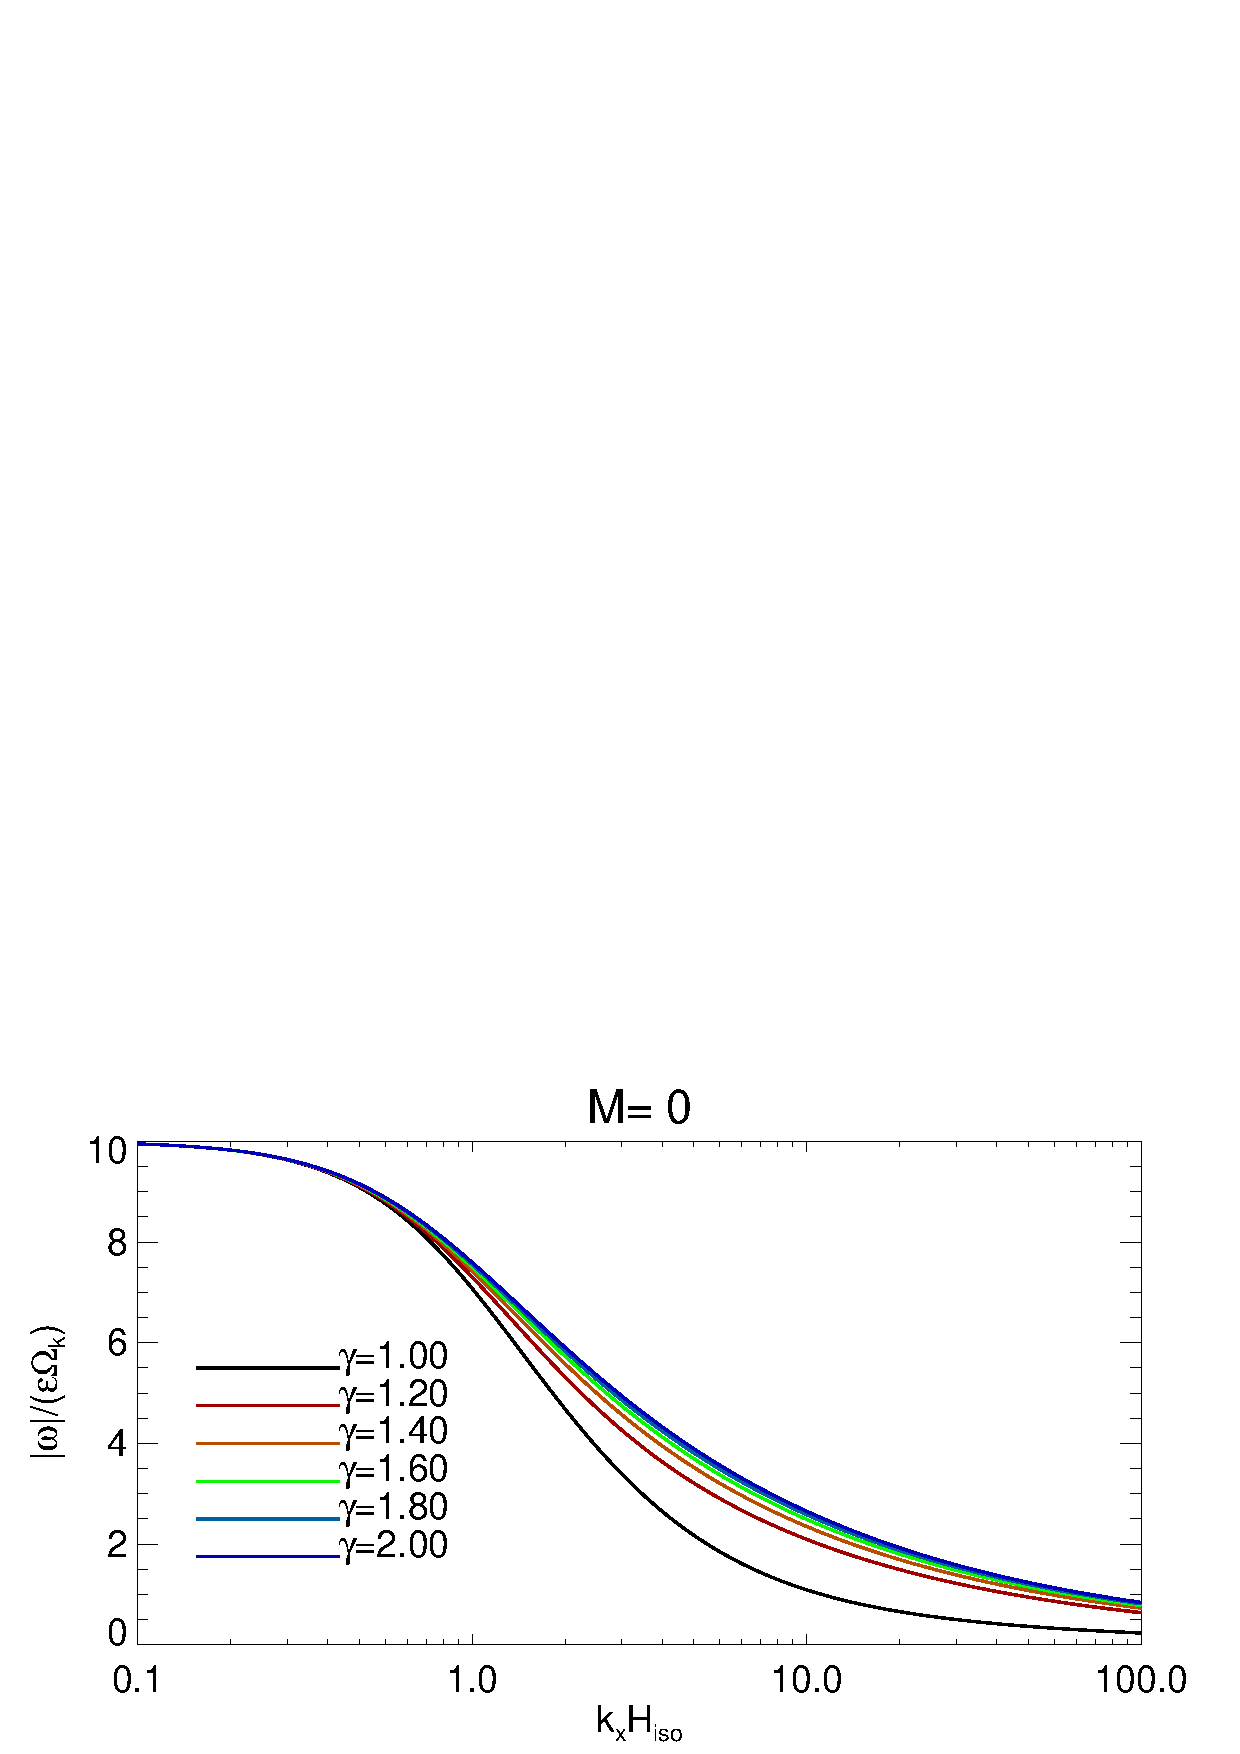
\includegraphics[width=\linewidth,clip=true,trim=0cm 1.75cm 0cm 0cm]{figures/rate_theory_om}
%   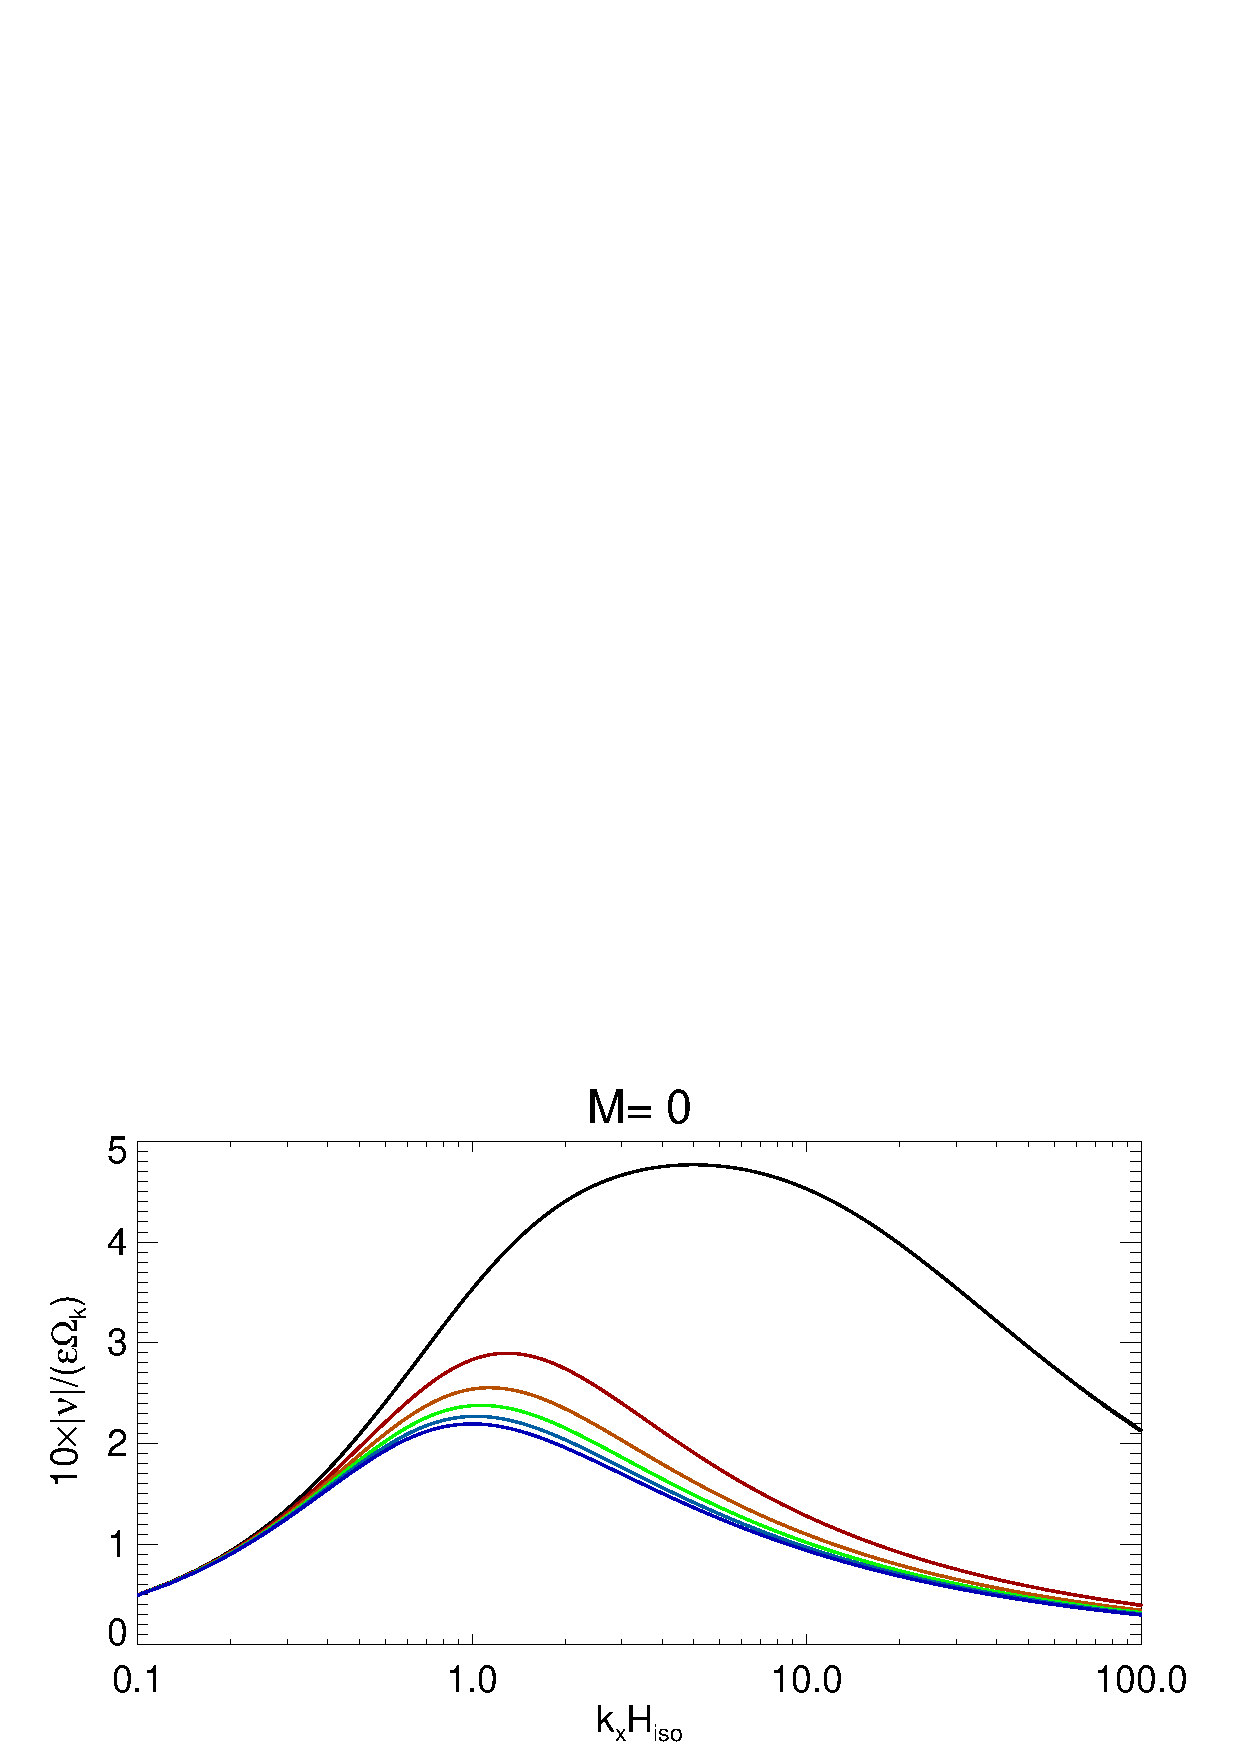
\includegraphics[width=\linewidth,clip=true,trim=0cm 0cm 0cm 1cm]{figures/rate_theory_nu}
%   \caption{Real frequency (top) and growth rate (bottom) of the fundamental VSI mode in vertically 
%     isothermal disks ($\Gamma=1$) subject to adiabatic perturbations,
%     calculated in thin disk approximation from Eq. \ref{adia_disp}
%     with $M=0$, $\epsilon=0.1$ and  
%     $|q|=1$. Frequencies are shown as a function of the radial
%     wavenumber for different values of the adiabatic index
%     $\gamma$. For $\gamma\equiv 1$ the perturbations are isothermal
%     and there is no vertical entropy gradient.\label{adia_growth}}  
% \end{figure}   
